\section{Tasking}


\subsection{Introduction}
The tasking elements of PEARL are mapped on the Posix thread library 
(\verb|pthread|) as far as possible. 
The pthread-library suffers in Linux from the absence of a \verb|suspend|-call.
Usually this is solved by doing a blocking systemcall in a signal handler and
invoke the corresponding signal.
This solutions works fine as long as no \verb|TERMINATE|-request is
issued to a suspended task. This will cause an abnormal program
termination --- terminating all threads. 
Thus a different approach is used. If a task should become suspended or terminated
by another task, the targeted task state is analysed.
If the task is running or blocked on i/o operation a flag is set
and the invoking task waits until the targeted task completes the request.
Additionally during i/o-operation, the targeted task is interrupted by the 
SIG\_CANCEL\_IO, which causes the system call to exit
with error code \verb|EINTR|. The system device driver must deal with this
situation. (refer \ref{linux_suspend}, \ref{linux_terminate})

\subsection{Task Control Block}
The task control block is represented by the attributes of the 
task-object. 
The task control block contains a Posix-semaphore to realize atomistic
operations on the tasks state variables.
A mutex appeared not to be sufficient, since
Posix mutex do no implicit reschedule in case of blocking and unblocking.
This would disturb the preemptive priority  paradigma of PEARL.

\subsection{SUSPEND-Operation}
\label{linux_suspend}
To suspend a task, the task waits for reception on a pipe.
The received characters are ether 'c' for continations or 't' for termination.
If a 't' is received the adressed task terminates itself.
Otherwise, the task continues its operation.





If the task should become suspended from itself or by another task, 
the situation is treated according the current task state by the
platform independent part and partially the operation is delegated 
to the platform specific part.

\begin{description}

\item[suspendMySelf] 
The self suspending is solved by a blocking \verb|read| on a pipe.
When the task should become continued,
 any other task may send the character 'c' onto the pipe.

\item[suspendRunning] the \verb|SUSPEND_PENDING| bit is set and the caller
   is blocked until this bit is recognized by the adressed task.
   The targeted task will be executed with best priority to avoid
   priority inversion.

%\item[BLOCKED on Semaphore, Bolt or IOWaitQueue]
%   the adressed task is removed from the
%   wait queue until it becomes continued. In this case the task is reinserted
%   in the according queue.
\item[suspendIO] the adressed task is interrupted by a 
   UNIX-signal (\verb|SIG_CANCEL_IO|). This causes the system
   call to become interrupted. This error condition EINTR must 
   be detected by the system device driver, which must invoke the method
   \verb|treatCancelIO()| of the current task. This method suspends 
   the task.
   The targeted task will be executed with best priority for this 
   action to avoid priority inversion.
   This action is common to all blocking system dations, thus this is 
   implemented in the classes \verb|InterruptableSystemDationNB| and
   \verb|InterruptableSystemDationB|.
\end{description}

The CONTINUE is delegated to the platform specific method
\verb|continueSuspended|.

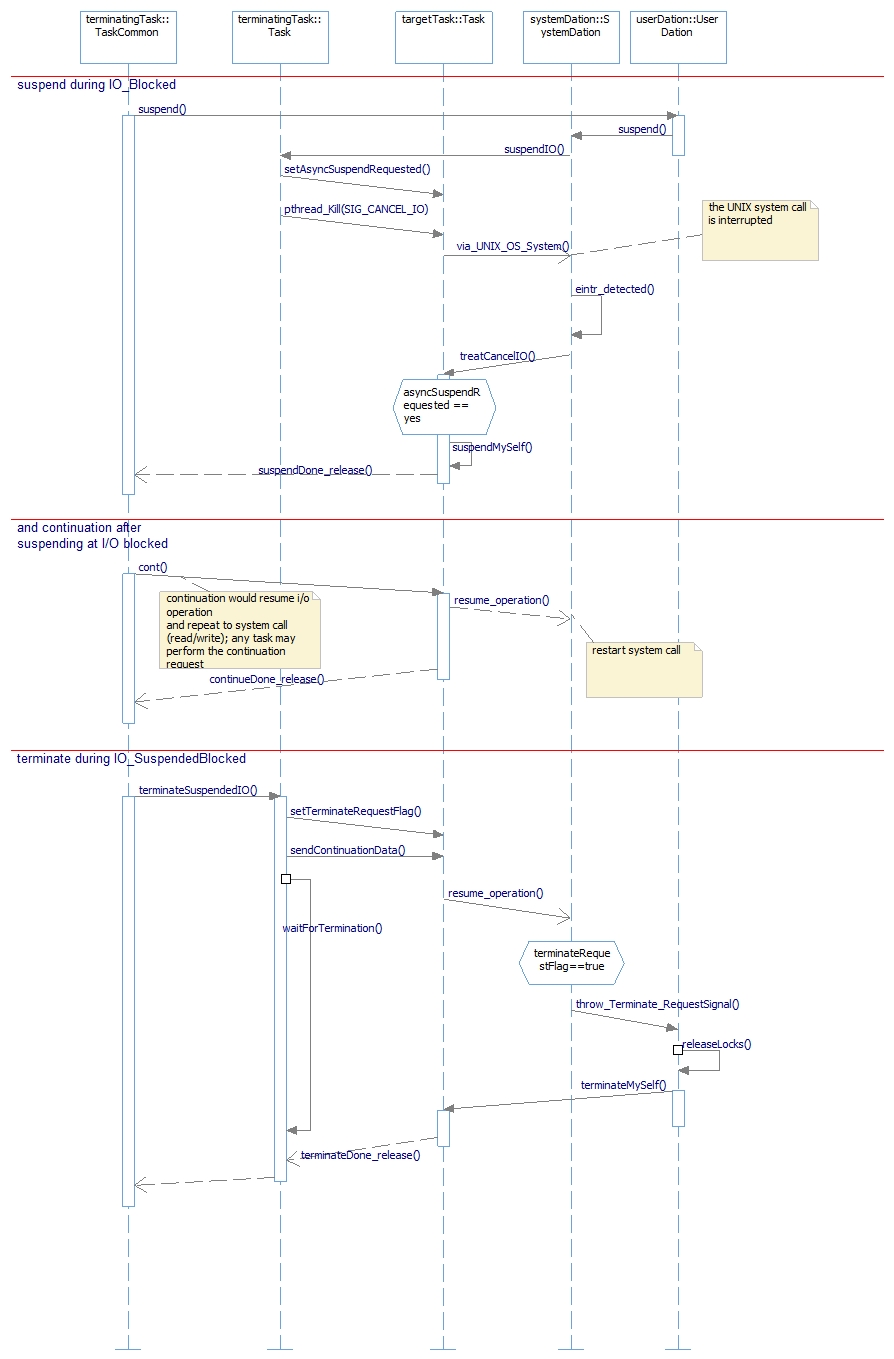
\includegraphics[width=15cm]{Linux_SuspendIO.jpg}


\subsection{TERMINATE Operation}
\label{linux_terminate}
A task may terminate itself or becomes terminated by another task.
The situation is treated according the current task state by the
platform independent part and partially the operation is delegated 
to the platform specific part.


\begin{description}
\item[terminateMySelf] The self termination is just a \verb|pthread_exit()|.
   If other task are waiting for a tasking method to finish (e.g. SUSPEND),
   they are informed that this is done.
   If there are other tasks waiting for the termination, they become
   unblocked just before the \verb|pthread_exit()| call.
   The targeted task will be executed with best priority to avoid
   priority inversion.
\item[terminateSuspended] emits just a 't' to the pipe of the task 
   to terminate.

\item[terminateSuspendedIO] set the \verb|asynTerminateRequested| flag
   and continue the suspended thread. This will detect the termination
   request and terminate self after unrolling the i/o stack

\item[terminateIO] the adressed task is interrupted by a 
   UNIX-signal (\verb|SIG_CANCEL_IO|). This causes the system
   call to become interrupted. This error condition EINTR must 
   be detected by the device driver, which must invoke the method
   \verb|treatCancelIO()| of the current task. This method emits the 
   exception \verb|TerminationRequestSignal|. This signal must be caught
   the device driver if cleanup actions are required. After cleanup,
   the signal must be emitted again to inform superior layers.
   The targeted task will be executed with best priority to avoid
   priority inversion. 
   The i/o-action finally catches the exception and terminates the task.
\end{description}

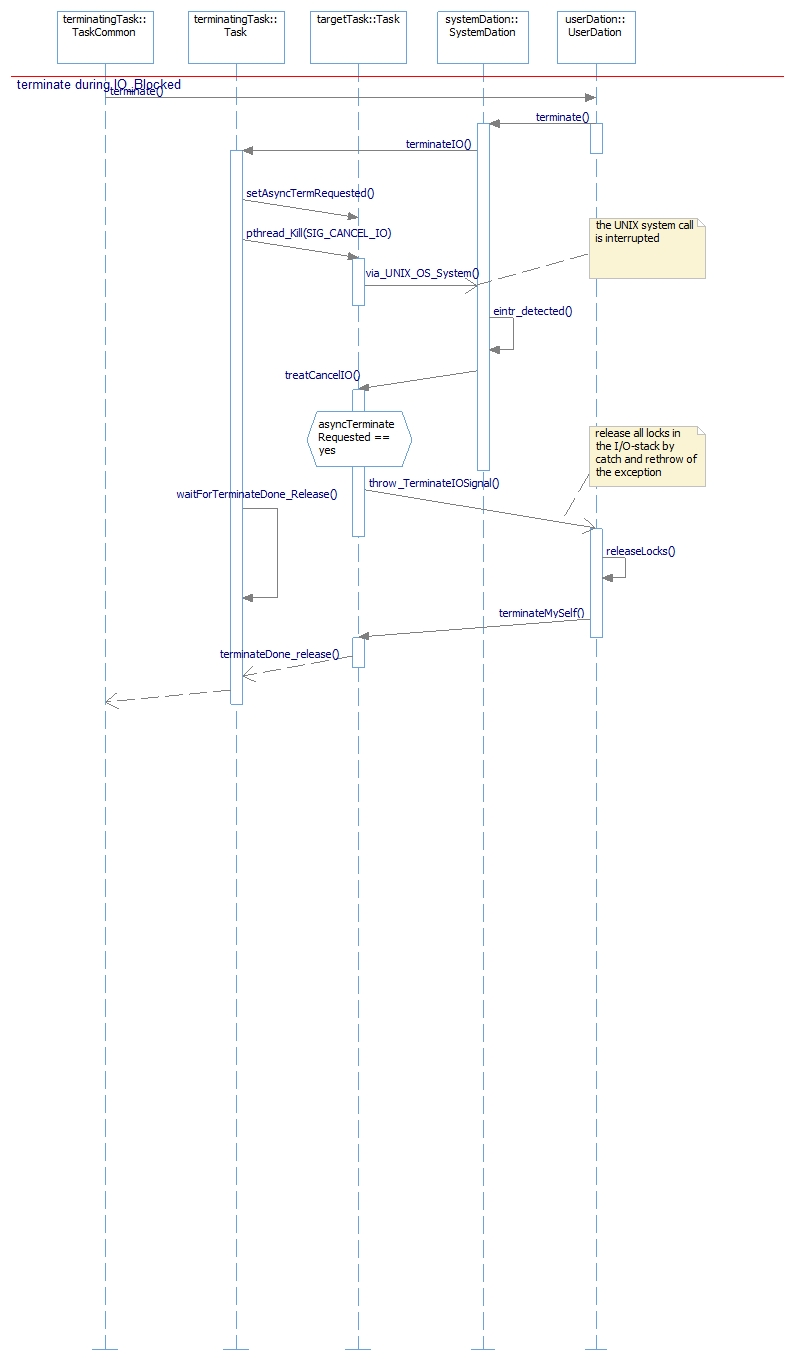
\includegraphics[width=15cm]{Linux_TerminateIO.jpg}



\subsection{Scheduled Operations (class TaskTimer)}
The scheduled operations like \verb|AFTER ... ACTIVATE| are realized with
Linux timers and realtime signals. 
The timers provide a start delay and repetition rate. This fits ideal to
the \verb|AFTER ... ALL ...| semantics.
The element \verb|AT| ist translated into \verb|AFTER| with respect of the current
time (\verb|NOW|).
The elements \verb|DURING| and \verb|until| are translated into a repetition 
counter. Each time the timer elapses a realtime signal is emitted.
The signal handler is treated inside the timer thread.
The handler decrements the counter.
When the counter reached 0, the timer will be stopped.

The real-time signals have the advantage that the reception is guaranteed.

There are independent timers for \verb|ACTIVATE|, \verb|CONTINUE| 
and \verb|RESUME|.

\paragraph{Remark:} Subsequent modification of the systems date and time 
will not affect the scheduled operation using \verb|AT| or \verb|UNTIL|.


\subsection{PrioMapper}
The Linux-scheduler {\em SCHED\_RR} supports 100 priorites. PEARL requieres 
256 different priorities.
The module {\em PrioMapper} maps PEARL-priorities to system priorities as good
as possible. The strategy is to map the best priorities in a 1:1 manner and the
worst priority to 99. 
Request with PEARL-priorities, which are not mappable result in a PEARL
signal raising.

The lowest and best priority is needed by the runtime system, thus 98 
priorities are avaiable for the OpenPEARL application.

If a different behavior is desired this module can be replaced or modified.


